\documentclass{beamer}

\usetheme{uhh}
\showtotalframenumber
\showuhhlogoeachframe
\showsections

\usepackage{amsmath}
\usepackage{graphicx}
\DeclareMathOperator*{\argmin}{arg\,min}

\usepackage{listings}
\lstset{
  language=python
  }

\title{Part 04: Implementing Word2Vec in Tensorflow}
\author{Fabian Barteld, Benjamin Milde}
\date[20.06.2016]{June 20, 2016}

\AtBeginSection[]
{
   %%%%% section title
   % This is how it would look like in Beamer:
   % \begin{frame}
   %     \frametitle{Overview}
   %     \tableofcontents[sections={2-3},currentsection,sectionstyle=show/hide,subsectionstyle=hide]
   % \end{frame}
  \begin{frame}[plain]
  \begin{tikzpicture}[overlay]
    \relax%
    \fill[blueuhh,opacity=1] (-10,-10)
    rectangle(\the\paperwidth,\the\paperheight);
  \end{tikzpicture}
   \begin{tikzpicture}[overlay]
    \relax%
    \fill[white,opacity=1] (-5,-1.2)
    rectangle(\the\paperwidth,0.5) node[pos=0.5,black]{\LARGE\insertsectionhead};
  \end{tikzpicture}
  \end{frame}

  %%%% add subsection to show navigation dots
  \subsection{}
}

\begin{document}

\maketitle

%\begin{frame}
%  \frametitle{Overview}
%
%  \tableofcontents
%
%\end{frame}

\section{Introduction}

\begin{frame}[fragile]
\frametitle{Training embeddings}
  \begin{itemize}
	\item We will now implement Word2Vec in Tensorflow
	\item (Slides smiliar to https://www.tensorflow.org/tutorials/word2vec)
	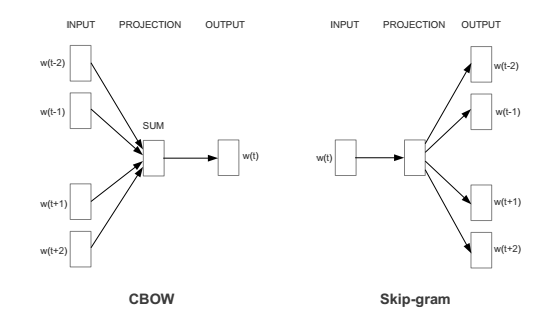
\includegraphics[width=0.7\textwidth]{04_skipgram_vs_cbow}
  \end{itemize}
\end{frame}

\begin{frame}
  \frametitle{Main concepts I}
  \begin{itemize}
     
    \item  Neural probabilistic language models are traditionally trained using the maximum likelihood (ML) principle (where $w_t$ is the target word and $h$ is the context):
	 
	 \end{itemize}

\begin{center}
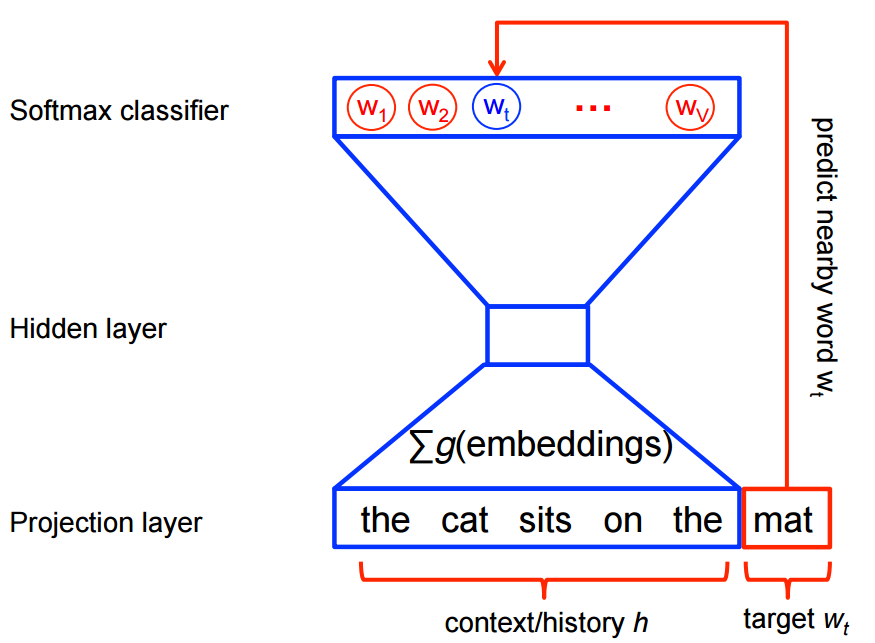
\includegraphics[width=0.5\textwidth]{04_w2v_01}
\end{center}	 
	 
\end{frame}

\begin{frame}
  \frametitle{Main concepts II}
  \begin{itemize}
     
    \item  Neural probabilistic language models are traditionally trained using the maximum likelihood (ML) principle (where $w_t$ is the target word and $h$ is the context):
	 
	 \end{itemize}

$$P(w_t | h) = \text{softmax}(\text{score}(w_t, h)) = $$
	$$ \frac{\ exp\{\text{score}(w_t, h) \} } {\sum_\text{Word w' in Vocab} \ exp\{ \text{score}(w', h) \}}$$	 
	 
\end{frame}

\begin{frame}
  \frametitle{Main concepts III}
  
    \begin{itemize}

	\item We train this model by maximizing its log-likelihood on the training set, i.e. by maximizing:

	$$  J_\text{ML} = \log P(w_t | h) \ = $$
	$$  \text{score}(w_t, h) - \log \left( \sum_\text{Word w' in Vocab} \exp { \text{score}(w', h) } \right). $$
	
	\item However this is very expensive, because we need to compute and normalize each probability using the score for all other $V$ words $w'$ in the current context $h$, at every training step.
	\end{itemize}
  
\end{frame} 

\begin{frame}
  \frametitle{Main concepts IV - NCE}
  
    \begin{itemize}
    \item Noise Contrastive Estimation (NCE)
	\item For feature learning in word2vec we do not need a full probabilistic model. Instead, we train to discriminate the real target words $w_t$ from $k$ imaginary (noise) words w~:
	
	\end{itemize}
	
	\begin{center}
	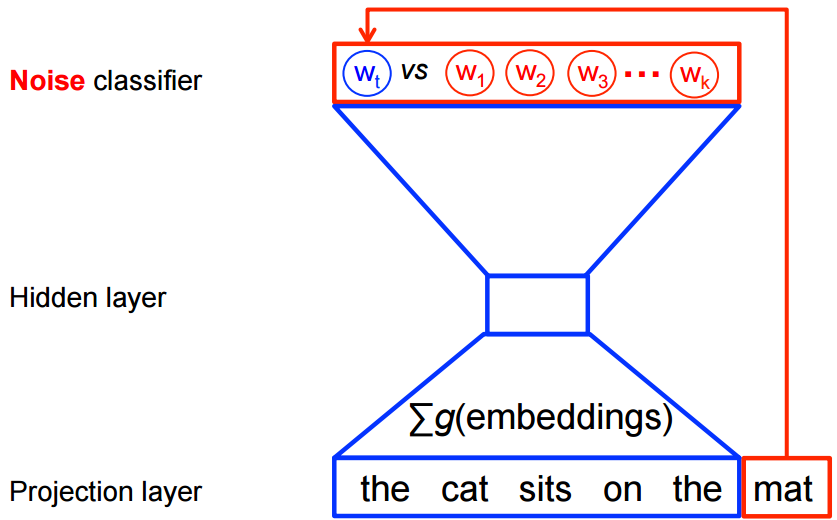
\includegraphics[width=0.6\textwidth]{04_w2v_02}
	\end{center}  
  
\end{frame} 


\begin{frame}
  \frametitle{Main concepts V - NCE}
  
  \begin{itemize}
\item Mathematically, the objective is to maximize:

$$J_\text{NCE} = \log Q_\theta(D=1 |w_t, h) + k \mathop{\mathbb{E}}\limits_{\tilde w \sim P_\text{noise}} \left[ \log Q_\theta(D = 0 |\tilde w, h) \right]$$

\item discriminate the real target words \(w_t\) from \(k\) imaginary (noise) words \(\tilde w\)
\item where $Q_\theta(D=1 | w, h)$ is the binary logistic regression probability
\item under the model of seeing the word $w$ in the context $h$ and assigning the label 1 for datapoint $D$, calculated in terms of the learned embedding vectors $\theta$

\end{itemize}
\end{frame} 

\begin{frame}
  \frametitle{Impl. I - Tensorflow W2V}
    \begin{itemize}
    	\item In practice we approximate the expectation by drawing k contrastive words from the noise distribution (i.e. we compute a Monte Carlo average) 
   $$J_\text{NCE} \approx \log Q_\theta(D=1 |w_t, h) +  \sum_{i=1, w \sim P_\text{noise}}^{k}  \left[ \log Q_\theta(D = 0 |\tilde w, h) \right]$$ 
   \item Now we can choose $k \neq |V|$, in practice 5-10 for small datasets, 2-5 for large datasets
   \item Negative sampling, as in the word2vec paper, is a variant of NCE and uses a specific distribution (uniform raised to the power of 3/4)
   
 \end{itemize}
\end{frame} 

\begin{frame}[fragile]
  \frametitle{Impl. II - Tensorflow W2V}
  \begin{lstlisting}

loss = tf.reduce_mean(
  tf.nn.nce_loss(weights=nce_weights,
                 biases=nce_biases,
                 labels=train_labels,
                 inputs=embed,
                 num_sampled=num_sampled,
                 num_classes=vocabulary_size))
    \end{lstlisting}
    
  \begin{itemize}
  	\item We can use the NCE loss op of Tensorflow to construct a variant of word2vec. Internally, nce\_weights also uses embedding\_lookup and does a form of negative sampling  directly in Tensorflow.
  \end{itemize}
\end{frame}
    
 \begin{frame}[fragile]
  \frametitle{Impl. III - Tensorflow W2V}
  The embeddings matrix is a variable that we want to optimize:
  \begin{lstlisting}
embeddings = tf.Variable(
tf.random_uniform([vocabulary_size,
embedding_size], -1.0, 1.0))
\end{lstlisting}    
\end{frame}

 \begin{frame}[fragile]
 \frametitle{Impl. IIII - Tensorflow W2V}
We also need variables for the nce\_loss:

\begin{footnotesize}
\begin{lstlisting}
nce_weights = tf.Variable(
  tf.truncated_normal([vocabulary_size, embedding_size],
stddev=1.0 / math.sqrt(embedding_size)))
nce_biases = tf.Variable(tf.zeros([vocabulary_size]))
\end{lstlisting}   
\end{footnotesize}    
\end{frame}

 \begin{frame}[fragile]
  \frametitle{Impl. IV - embedding\_lookup:}
  
  \begin{footnotesize}
 \begin{lstlisting}
embed = tf.nn.embedding_lookup(embeddings, train_inputs)
\end{lstlisting}
\end{footnotesize}    

e.g. If your list of sentences is: $\big[[0, 1], [0, 3]\big]$ (sentence 1 is $[0, 1]$, sentence 2 is $[0, 3]$, the function will compute a tensor of embeddings, which will be of shape $(2, 2, \text{embedding\_size})$ and will look like:
\\
$$[[\text{embedding0, embedding1}], [\text{embedding0, embedding3}]]$$

\end{frame}

 \begin{frame}[fragile]

  \frametitle{Exercise 1 - simple version}
   \begin{itemize}
   		\item Lets put it together: We can use tf.nn.embedding\_lookup for the input projection and tf.nn.nce\_loss for the loss (no other layers needed!).
		\item For simplicity, lets also implement CBOW and Skipgram with a window size of 1. 
		\item E.g. for "the quick brown fox jumped over the lazy dog"
		\item (context, target) pairs: ([the, brown], quick), ([quick, fox], brown), ([brown, jumped], fox)
		\item We can simplify to: (the, quick), (brown, quick), (quick, brown), (fox, brown), ... \textbf{CBOW}
		\item or (quick, the), (quick, brown), (brown, quick), (brown, fox), ... \textbf{Skip-gram}
	\end{itemize}
\end{frame}

 \begin{frame}[fragile]

  \frametitle{Exercise 2 - advanced version}
   \begin{itemize}
		\item Lets try to make a version that does not use tf.nn.nce\_loss, as easy as that makes our lives!
		\item We can also do the negative sampling on the host and code up a linear regression as in the previous tutorials
		\item Host will assign labels (1 for true context pairs, 0 for noise pairs)
		\item You have to change the code in the get\_batch function and the inputs to your model and adapt your model accordingly		
	\end{itemize}
\end{frame}

 \begin{frame}[fragile]
 
 \frametitle{Hints}
  \begin{itemize}
		\item Hint1: The negative samples need a second embedding matrix
		\item Hint2: For the loss, to get the logits, use the dot product between embedding pairs.
		\item Hint3: There is no tf.dot(), but you can combine tf.reduce\_sum(x,1) and tf.multiply(a,b).
		\item Hint4: Readable pure Python code with comments: , or if you're feeling masochistic the original uncommented word2vec C impl at: 
	\end{itemize}
		
\end{frame}


 \begin{frame}[fragile]
 
 \frametitle{Tensorboard}
  \begin{itemize}
		\item Visualize loss, embeddings and much more in your browser
		\item You need to add a few lines of code to tell Tensorboard what to log
		\item Make sure train\_summary\_dir is a new directory for every new experiment!
	\end{itemize}
			
	\begin{tiny}
\begin{lstlisting}
 loss_summary = tf.summary.scalar('loss', loss) 
 train_summary_op = tf.summary.merge_all()
 summary_writer = tf.summary.FileWriter(train_summary_dir, sess.graph)
\end{lstlisting}   
\end{tiny}    
	
\end{frame}

\begin{frame}[fragile]
 
 \frametitle{Tensorboard}
  \begin{itemize}
		\item You need to regularly call the train\_summary\_op in training
		\item Not as often as the training step, because it will otherwise slowdown your training if you have more complex summaries
	\end{itemize}
			
\begin{tiny}
\begin{lstlisting}
if current_step % 100==0 and current_step != 0:
	summary_str = sess.run(train_summary_op, feed_dict=feed_dict)
	summary_writer.add_summary(summary_str, current_step)
\end{lstlisting}   
\end{tiny}    
	
\end{frame}

\begin{frame}[fragile]
 \frametitle{Tensorboard - running it}
 \begin{tiny}
 \begin{lstlisting}
python3 -m tensorflow.tensorboard  --logdir=w2v_summaries_1499773534
--host=127.0.0.1
\end{lstlisting}   
\end{tiny}
 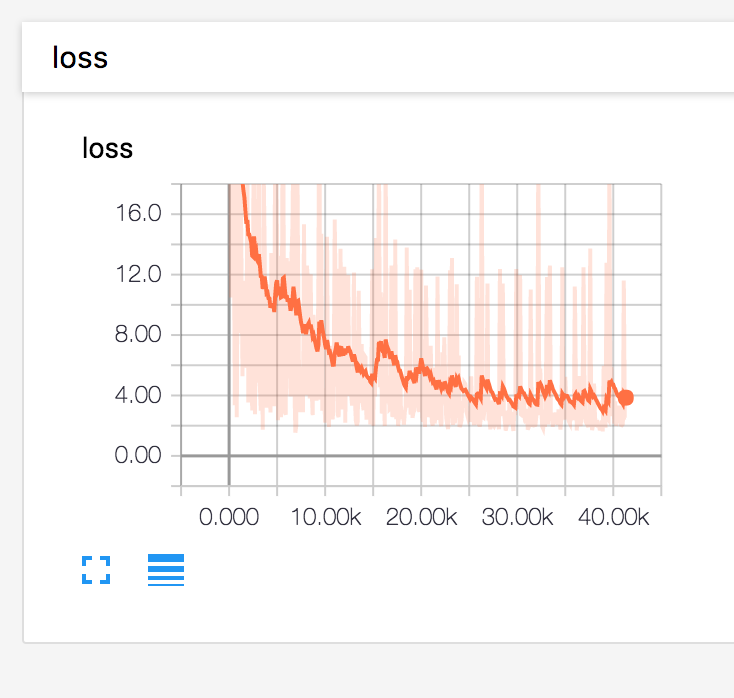
\includegraphics[width=0.5\textwidth]{04_loss}
\end{frame}


\begin{frame}[fragile]
 \frametitle{Tensorboard - embeddings}
   \begin{itemize}
		\item Possible to nicely visualize embeddigs, see \url{https://www.tensorflow.org/get_started/embedding_viz}
		\item Also checkout \url{http://projector.tensorflow.org/}, live demo of pretrained embeddings
		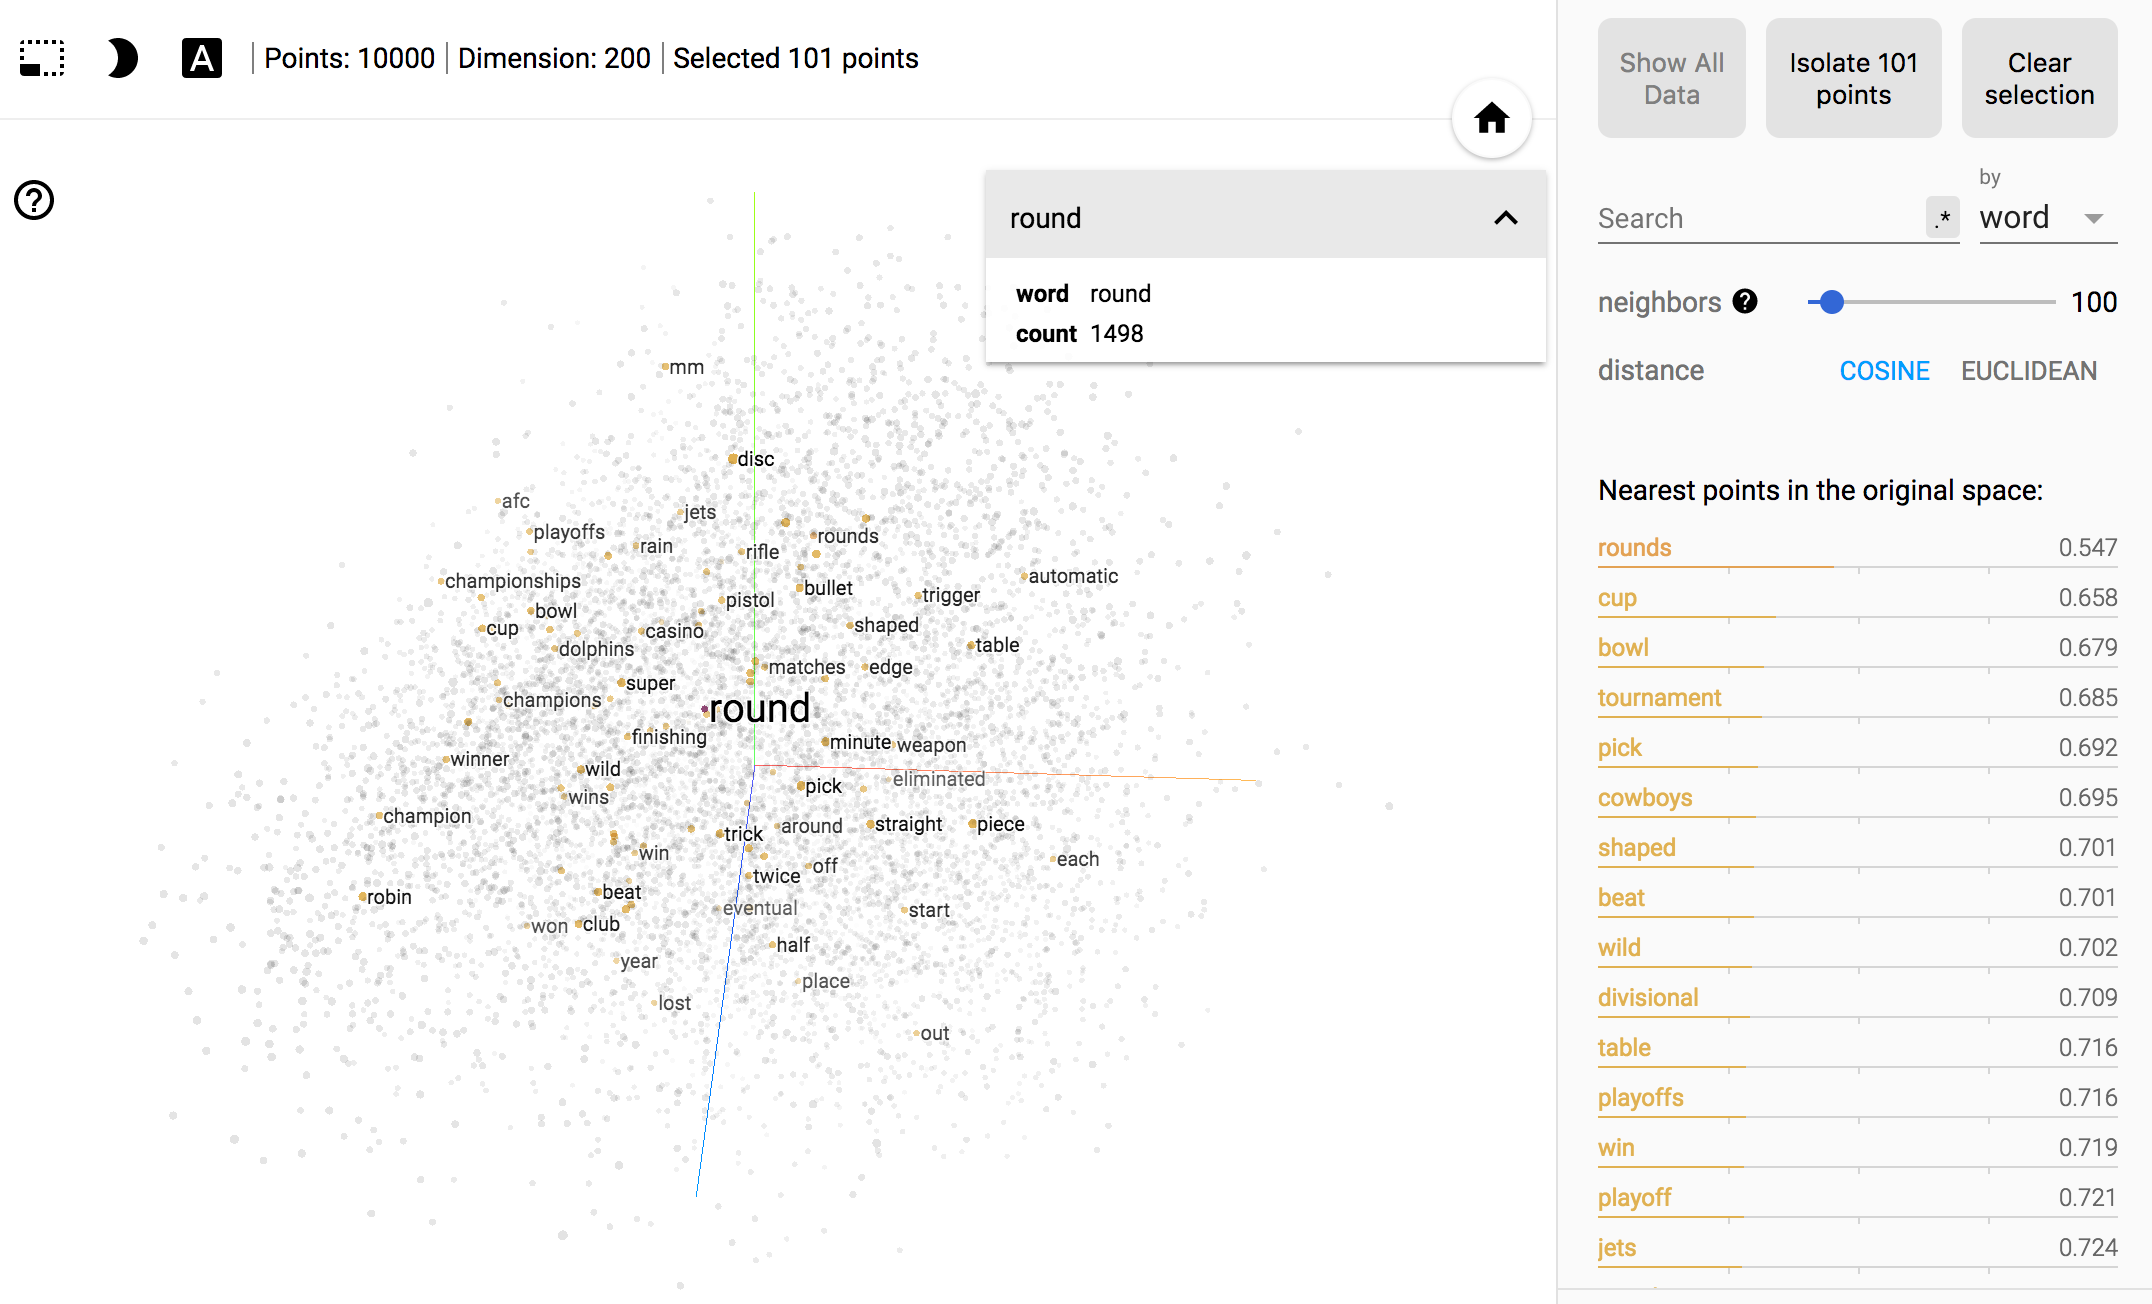
\includegraphics[width=0.5\textwidth]{04_embed_viz.png}
	\end{itemize}
\end{frame}

 
%\begin{frame}[fragile]
%  \frametitle{Layer based APIs vs. Graphs based}
%  
%Disadvantage: Difficult to express structures like these:
%  
%    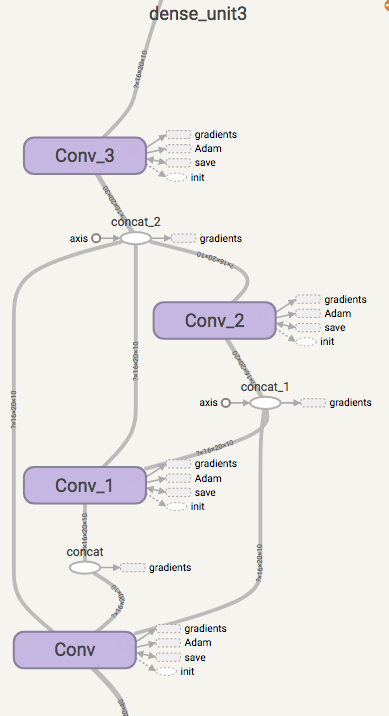
\includegraphics[angle=-90,width=0.75\textwidth]{graph_example}
%
%Increasing evidence that these kind of deeply connected networks are very useful.
%  
%\end{frame} 
%
%\begin{frame}[fragile]
%  \frametitle{Layer based APIs vs. Graphs based}
%  \begin{itemize}
%		\item  Since Tensorflow uses computation graphs, the declaration of the model allows for a higher expressivity
%		\item  Has a steeper learning curve in the beginning
%		\item  In the newer versions of tensorflow, you can also mix layer-like APIs with the computation graph
%		\item  We will focus on not using any short cuts, as this has a higher learning effect and only make use of standard ops in the beginning
%  \end{itemize}
%\end{frame} 
%
%\begin{frame}[fragile]
%\frametitle{First steps - Lets open spyder}
%
%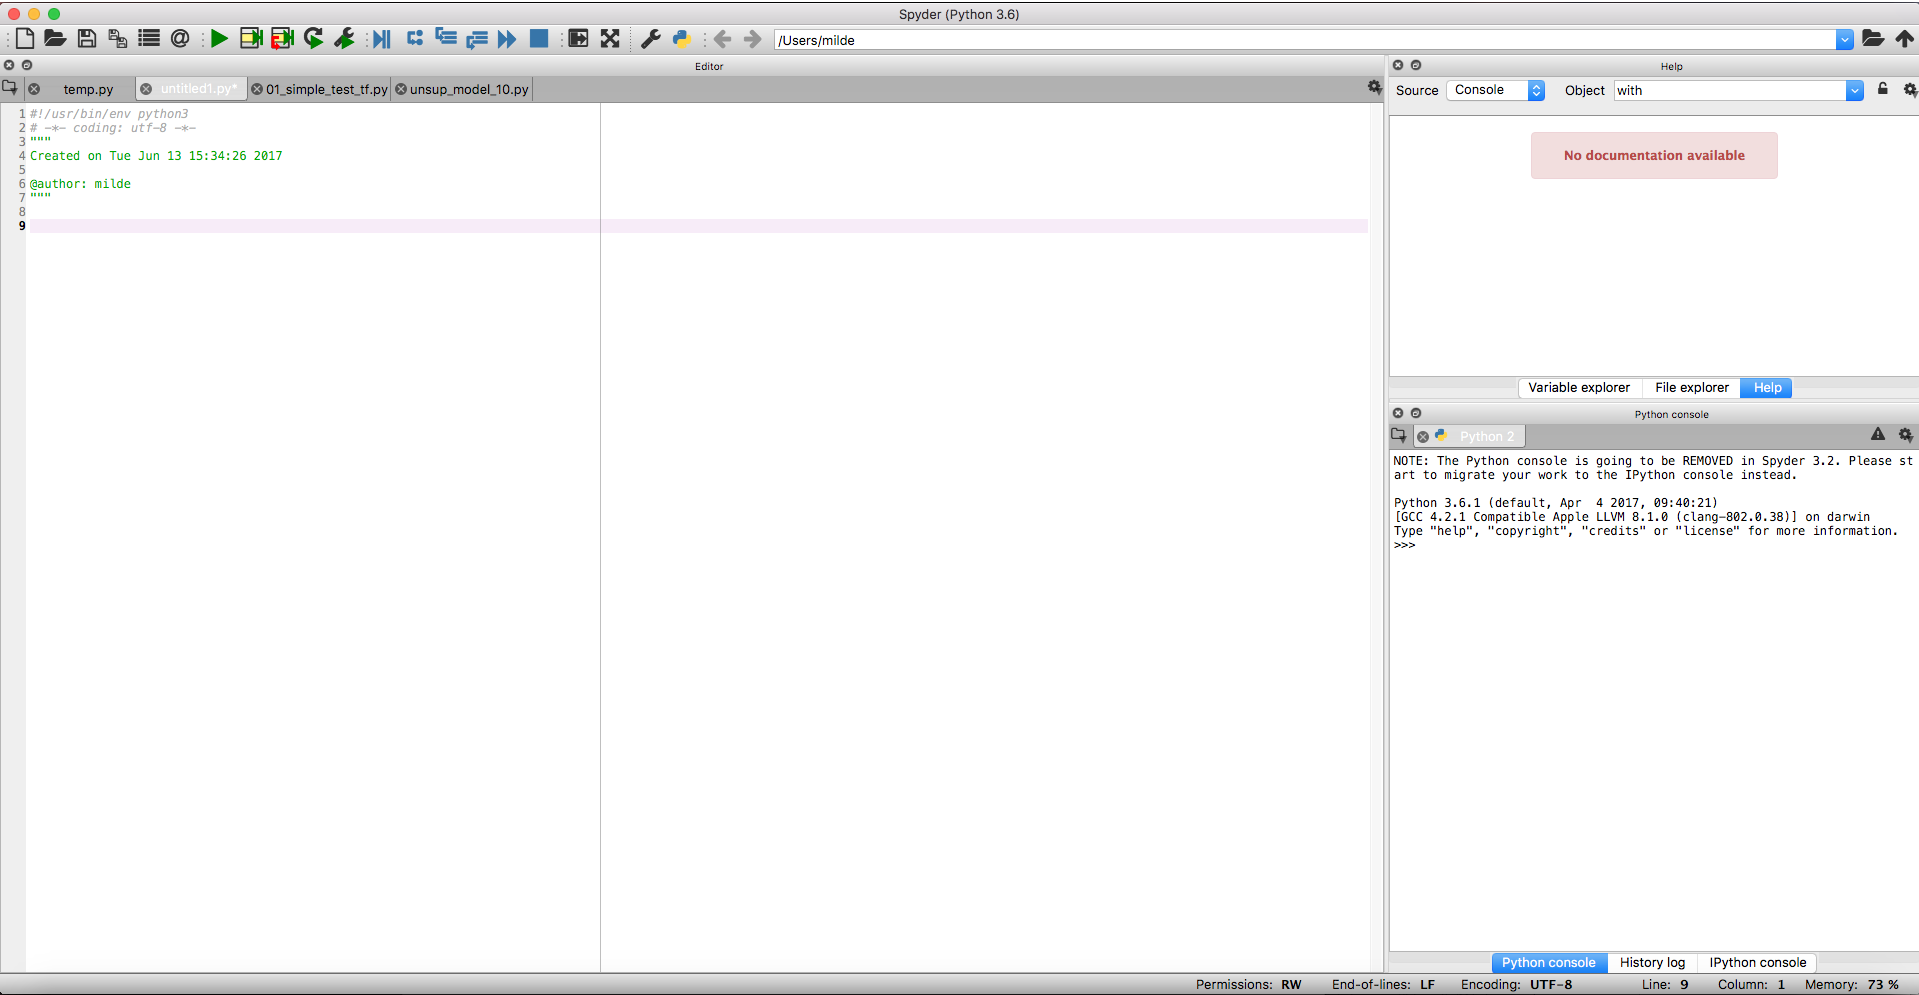
\includegraphics[width=1.0\textwidth]{spyder}
%
%\end{frame} 
%
%\begin{frame}[fragile]
%\frametitle{First steps - Necessary imports}
%
%\begin{lstlisting}
%import numpy as np
%import tensorflow as tf
%\end{lstlisting}
%
%\begin{itemize}
% 	\item Outside of graph computations, we usually store data in Numpy arrays.
% 	\item Numpy arrays are the main objects to transfer data to inputs of the graph and from outputs of the graph.
% 	\item Numpy arrays are also an abstraction for (homogeneous) multidimensional arrays.
%\end{itemize}
%
%\end{frame} 
%
%\begin{frame}[fragile]
%\frametitle{Generating some random data}
%
%\begin{lstlisting}
%#some random test data
%a_data = np.random.rand(256)
%b_data = np.random.rand(256)
%\end{lstlisting}
%
%\begin{itemize}
%	\item Now a and b contain vectors of length 256 with random floats. E.g. print(a\_data) returns:
%\end{itemize}
%
%\begin{lstlisting}
%[ 0.54976368  0.87790201  0.96528541 ..., 
% 0.05281365  0.48556404  0.46848266]
%  \end{lstlisting}
%
%\end{frame} 
%
%
%\begin{frame}[fragile]
%\frametitle{Declare the computation graph}
%
%\begin{lstlisting}
%#construct the graph
%a = tf.placeholder(tf.float32, [256])
%b = tf.placeholder(tf.float32, [256])
%
%x = a+b 
%\end{lstlisting}
%
%\begin{itemize}
%\item The placeholders can later be used to input data to the computation graph
%\item The operation x = a+b does not immediatly add something, it creates a graph.
%\item In fact, print(x) returns: 
%\end{itemize}
%
%\begin{lstlisting}
%Tensor("add:0", shape=(256,), dtype=float32)
%\end{lstlisting}
%
%\end{frame} 
%
%\begin{frame}[fragile]
%\frametitle{A session on a computation device}
%
%\begin{lstlisting}
%with tf.device('/cpu'):
%    with tf.Session() as sess:
%       x_data = sess.run(x, {a: a_data, b: b_data})  
%       print(x_data)
%\end{lstlisting}
%
%\begin{itemize}
%\item This fills the inputs a and b with a\_data and b\_data (our random data), runs the computation graph and retrieves the results of x in x\_data
%\item Obviously not terrible useful as is, but you could run the operation easily on a gpu by changing tf.device('/cpu') to  tf.device('/gpu:1'). Copying data to and from the GPU is handled automatically for you.
%\end{itemize}
%
%\end{frame} 
%
%\begin{frame}[fragile]
%\frametitle{Small warm up exercise!}
%
%\begin{itemize}
%	\item We change a and b to random matrices:
%\end{itemize}
%
%\begin{lstlisting}
%a = np.random.rand(256, 128)
%b = np.random.rand(128, 512)
%\end{lstlisting}
%
%\begin{itemize}
%	\item Calculate the resulting matrix of shape (256, 512) in TensorFlow.
%\end{itemize}
%
%\end{frame} 

%\section{Simple Optimization}
%
%% https://medium.com/@saxenarohan97/intro-to-tensorflow-solving-a-simple-regression-problem-e87b42fd4845
%% https://github.com/aymericdamien/TensorFlow-Examples/blob/master/examples/2_BasicModels/linear_regression.py
%\begin{frame}
%  \frametitle{Linear Regression}
%
%  \begin{itemize}
%  \item Given: $(x_1, y_1)$, \ldots, $(x_n,y_n)$
%  \item Goal: find $w$ and $b$ such that:
%    \begin{displaymath}
%      \argmin_{w, b} \frac{\sum^n_{i=1} (\hat{y}_i - y_i)^2}{n}
%    \end{displaymath}
%    where $\hat{y}_i = wx_i + b$.
%  \end{itemize}
%
%\end{frame}
%
%\begin{frame}[fragile]
%  \frametitle{Define model parameters}
%  Model: $\hat{y}_i = wx_i + b$
%
%\begin{lstlisting}
%w = tf.Variable(np.random.randn(), name="weight")
%b = tf.Variable(np.random.randn(), name="bias")
%\end{lstlisting}
%\end{frame}
%
%\begin{frame}[fragile]
%  \frametitle{Define the model}
%
%  \begin{displaymath}
%    \begin{pmatrix} \hat{y}_1\\\vdots\\\hat{y}_n\end{pmatrix} =
%    \begin{pmatrix} w\\\vdots\\w\end{pmatrix} *
%    \begin{pmatrix} \hat{x}_1\\\vdots\\\hat{x}_n\end{pmatrix} +
%    \begin{pmatrix} b\\\vdots\\b\end{pmatrix}
%  \end{displaymath}
%
%\begin{lstlisting}
%yhat = tf.add(tf.multiply(X, w), b)
%\end{lstlisting}
%
%{\footnotesize The scalars $w$ and $b$ are converted into vectors of the same
%  length as X (broadcast); \url{https://www.tensorflow.org/performance/xla/broadcasting}}
%
%\end{frame}
%
%\begin{frame}[fragile]
%  \frametitle{Define the loss}
%
%\begin{lstlisting}
%loss = tf.reduce_mean(tf.square(y - yhat))
%\end{lstlisting}
%
%\end{frame}
%
%
%\begin{frame}[fragile]
%  \frametitle{Optimization}
%
%\begin{lstlisting}
%epochs = 10
%optimizer = tf.train.GradientDescentOptimizer(
%    learning_rate).minimize(loss)
%
%with tf.Session() as sess:
%    ## initalize parameters
%    sess.run(tf.global_variables_initializer())
%
%    for i in list(range(epochs)):
%        ## run one epoch
%        sess.run(optimizer)
%        ## print result and loss
%        print(sess.run(yhat) + ' ' + sess.run(loss))
%\end{lstlisting}
%
%\end{frame}
%
%\begin{frame}[fragile]
%  \frametitle{Hands on: Simple optimization}
%
%  \begin{enumerate}
%  \item Do a linear regression to learn $y = 2x + 1$
%  \item Do a multiple linear regression with Boston housing prices
%  \end{enumerate}
%
%\begin{lstlisting}
%from sklearn.datasets import load_boston
%from sklearn.preprocessing import scale
%
%total_X, total_Y = load_boston(True)
%total_x = scale(total_x)
%\end{lstlisting}
%\end{frame}
%
%% https://www.tensorflow.org/tutorials/wide
%% https://github.com/aymericdamien/TensorFlow-Examples/blob/master/examples/2_BasicModels/logistic_regression.py
%\begin{frame}
%  \frametitle{Logistic regression}
%
%  TODO
%  tf.sigmoid
%
%\end{frame}
%
%\begin{frame}
%  \frametitle{Hands on: Regression model}
%
%  TODO: more complex example
%\end{frame}

\end{document}


%%% Local Variables:
%%% mode: latex
%%% TeX-engine: luatex
%%% End:
